\documentclass[11pt,a4paper]{article}

% ============================================================================
% PACKAGE IMPORTS
% ============================================================================

% Font and encoding
\usepackage[utf8]{inputenc}
\usepackage[T1]{fontenc}
\usepackage{lmodern}
\usepackage{microtype}

% Language and typography
\usepackage[english]{babel}
\usepackage{csquotes}

% Page layout and geometry
\usepackage[margin=1in, paperheight=19.5in, paperwidth=8.5in]{geometry}
\usepackage{setspace}
\usepackage{parskip}

% Mathematics
\usepackage{amsmath}
\usepackage{amssymb}
\usepackage{amsthm}
\usepackage{mathtools}
\usepackage{bm}

% Graphics and figures
\usepackage{graphicx}
\usepackage{tikz}
\usetikzlibrary{positioning}
\usepackage{pgfplots}
\usepackage{subcaption}
\usepackage{float}
\usepackage{wrapfig}

% Colors and styling
\usepackage{xcolor}
\usepackage{tcolorbox}
\usepackage{mdframed}
\usepackage{framed}

% Tables
\usepackage{booktabs}
\usepackage{tabularx}
\usepackage{multirow}
\usepackage{array}

% Lists and enumeration
\usepackage{enumitem}

% Code and algorithms
\usepackage{listings}
\usepackage[ruled,vlined]{algorithm2e}

% References and links
\usepackage{hyperref}
\usepackage{cleveref}
\usepackage{url}

% Headers and footers
\usepackage{fancyhdr}
\usepackage{lastpage}

% Bibliography
\usepackage[backend=biber,style=alphabetic,sorting=ynt]{biblatex}

% ============================================================================
% COLOR DEFINITIONS
% ============================================================================

\definecolor{primaryblue}{RGB}{41, 128, 185}
\definecolor{secondaryblue}{RGB}{52, 152, 219}
\definecolor{darkblue}{RGB}{44, 62, 80}
\definecolor{lightblue}{RGB}{174, 214, 241}
\definecolor{accentorange}{RGB}{230, 126, 34}
\definecolor{accentgreen}{RGB}{46, 125, 50}
\definecolor{accentred}{RGB}{231, 76, 60}
\definecolor{lightgray}{RGB}{236, 240, 241}
\definecolor{darkgray}{RGB}{84, 110, 122}
\definecolor{codegray}{RGB}{248, 249, 250}

% ============================================================================
% HYPERREF SETUP
% ============================================================================

\hypersetup{
    colorlinks=true,
    linkcolor=primaryblue,
    filecolor=primaryblue,
    urlcolor=primaryblue,
    citecolor=primaryblue,
    bookmarksopen=true,
    bookmarksnumbered=true,
    pdfstartview={FitH},
    pdfauthor={Zejd Murat},
    pdftitle={Deep Learning with Andrew Ng - Study Notes},
    pdfsubject={Deep Learning},
    pdfkeywords={Deep Learning, Machine Learning, Neural Networks, Andrew Ng}
}

% ============================================================================
% CUSTOM ENVIRONMENTS
% ============================================================================

% Theorem-like environments
\theoremstyle{definition}
\newtheorem{definition}{Definition}[section]
\newtheorem{theorem}{Theorem}[section]
\newtheorem{lemma}{Lemma}[section]
\newtheorem{corollary}{Corollary}[section]
\newtheorem{proposition}{Proposition}[section]

\theoremstyle{remark}
\newtheorem{remark}{Remark}[section]
\newtheorem{example}{Example}[section]
\newtheorem{note}{Note}[section]

% Custom colored boxes
\tcbuselibrary{theorems}

% Key Concept Box
\newtcolorbox{keyconcept}{
    colback=lightblue,
    colframe=primaryblue,
    fonttitle=\bfseries,
    title=Key Concept,
    rounded corners,
    boxrule=1pt,
    left=8pt,
    right=8pt,
    top=8pt,
    bottom=8pt
}

% Important Formula Box
\newtcolorbox{formula}{
    colback=lightgray,
    colframe=darkgray,
    fonttitle=\bfseries,
    title=Important Formula,
    rounded corners,
    boxrule=1pt,
    left=8pt,
    right=8pt,
    top=8pt,
    bottom=8pt
}

% Gradient Computation Box
\newtcolorbox{gradcomp}{
    colback=lightgray,
    colframe=darkgray,
    fonttitle=\bfseries,
    title=Gradient Computation,
    rounded corners,
    boxrule=1pt,
    left=8pt,
    right=8pt,
    top=8pt,
    bottom=8pt
}

% Warning/Attention Box
\newtcolorbox{attention}{
    colback=accentorange!10,
    colframe=accentorange,
    fonttitle=\bfseries,
    title=Attention,
    rounded corners,
    boxrule=1pt,
    left=8pt,
    right=8pt,
    top=8pt,
    bottom=8pt
}

% Intuition Box
\newtcolorbox{intuition}{
    colback=accentgreen!10,
    colframe=accentgreen,
    fonttitle=\bfseries,
    title=Intuition,
    rounded corners,
    boxrule=1pt,
    left=8pt,
    right=8pt,
    top=8pt,
    bottom=8pt
}

% Follow-up Box
\newtcolorbox{followup}{
    colback=secondaryblue!10,
    colframe=secondaryblue,
    fonttitle=\bfseries,
    title=Follow-up,
    rounded corners,
    boxrule=1pt,
    left=8pt,
    right=8pt,
    top=8pt,
    bottom=8pt
}

% ============================================================================
% CUSTOM COMMANDS
% ============================================================================

% Common math operators
\DeclareMathOperator{\sigmoid}{sigmoid}
\DeclareMathOperator{\softmax}{softmax}
\DeclareMathOperator{\relu}{ReLU}
\DeclareMathOperator{\mytanh}{tanh}
\DeclareMathOperator{\argmax}{argmax}
\DeclareMathOperator{\argmin}{argmin}
\DeclareMathOperator{\trace}{tr}
\DeclareMathOperator{\diag}{diag}
\DeclareMathOperator{\rank}{rank}
\DeclareMathOperator{\var}{Var}
\DeclareMathOperator{\cov}{Cov}
\DeclareMathOperator{\mybias}{Bias}

% Vectors and matrices
\newcommand{\vect}[1]{\bm{#1}}
\newcommand{\mat}[1]{\bm{#1}}
\newcommand{\trans}[1]{#1^{\top}}
\newcommand{\inv}[1]{#1^{-1}}

% Probability and statistics
\newcommand{\prob}[1]{\mathbb{P}\left(#1\right)}
\newcommand{\expect}[1]{\mathbb{E}\left[#1\right]}
\newcommand{\given}{\mid}
\newcommand{\normal}[2]{\mathcal{N}\left(#1, #2\right)}

% Common sets
\newcommand{\reals}{\mathbb{R}}
\newcommand{\naturals}{\mathbb{N}}
\newcommand{\integers}{\mathbb{Z}}
\newcommand{\rationals}{\mathbb{Q}}
\newcommand{\complex}{\mathbb{C}}

% Neural network notation
\newcommand{\layer}[1]{^{[#1]}}
\newcommand{\activation}[2]{a\layer{#1}_{#2}}
\newcommand{\weight}[2]{W\layer{#1}_{#2}}
\newcommand{\nbias}[1]{b\layer{#1}}
\newcommand{\cost}[1]{J\left(#1\right)}
\newcommand{\gradient}[2]{\frac{\partial #1}{\partial #2}}

% ============================================================================
% LISTINGS SETUP FOR CODE
% ============================================================================

\lstset{
    basicstyle=\ttfamily\small,
    backgroundcolor=\color{codegray},
    commentstyle=\color{darkgray},
    keywordstyle=\color{primaryblue}\bfseries,
    numberstyle=\tiny\color{darkgray},
    stringstyle=\color{accentorange},
    breakatwhitespace=false,
    breaklines=true,
    captionpos=b,
    keepspaces=true,
    numbers=left,
    numbersep=5pt,
    showspaces=false,
    showstringspaces=false,
    showtabs=false,
    tabsize=2,
    frame=single,
    rulecolor=\color{lightgray},
    xleftmargin=0.5cm,
    xrightmargin=0.5cm,
    aboveskip=10pt,
    belowskip=10pt
}

% ============================================================================
% HEADER AND FOOTER SETUP
% ============================================================================

\setlength{\headheight}{25pt}
\pagestyle{fancy}
\fancyhf{}
\fancyhead[L]{\textcolor{primaryblue}{\textbf{Deep Learning Study Notes}}}
\fancyhead[R]{\textcolor{darkgray}{\thepage\ of \pageref{LastPage}}}
\fancyfoot[C]{\textcolor{darkgray}{\small Andrew Ng Course}}
\renewcommand{\headrulewidth}{1pt}
\renewcommand{\footrulewidth}{0.5pt}
\renewcommand{\headrule}{\hbox to\headwidth{\color{primaryblue}\leaders\hrule height \headrulewidth\hfill}}
\renewcommand{\footrule}{\hbox to\headwidth{\color{lightgray}\leaders\hrule height \footrulewidth\hfill}}

% ============================================================================
% TITLE PAGE SETUP
% ============================================================================

\title{
    \vspace{-1in}
    \begin{flushleft}
    \huge\textbf{\textcolor{primaryblue}{Deep Learning}} \\
    \Large\textcolor{darkgray}{Comprehensive Study Notes} \\
    \vspace{0.2cm}
    \large\textcolor{accentorange}{Andrew Ng Course} \\
    \end{flushleft}
    \vspace{-0.8in}
}

\author{}
\date{}

% ============================================================================
% DOCUMENT SETTINGS
% ============================================================================

\setlength{\parindent}{0pt}
\setlength{\parskip}{0.5em}
\onehalfspacing

% Adjust section spacing
\usepackage{titlesec}
\titleformat{\section}
    {\Large\bfseries\color{primaryblue}}
    {\thesection}
    {1em}
    {}
    [\color{primaryblue}\titlerule]

\titleformat{\subsection}
    {\large\bfseries\color{darkblue}}
    {\thesubsection}
    {1em}
    {}

\titleformat{\subsubsection}
    {\normalsize\bfseries\color{darkgray}}
    {\thesubsubsection}
    {1em}
    {}

% ============================================================================
% DOCUMENT BEGINS
% ============================================================================

\begin{document}

\maketitle

\vspace{0.3cm}

\begin{keyconcept}
\textbf{Welcome to my Deep Learning journey!} \\
This document serves as my study companion for Andrew Ng's Deep Learning course.
\end{keyconcept}

\vspace{0.3cm}

\tableofcontents

\newpage

% ============================================================================
% LOGISTIC REGRESSION
% ============================================================================

\begin{attention}
\textbf{Classical ML vs Deep Learning:} \\
One main difference between "classical" machine learning algorithms and deep learning algorithms is that Deep Learning models "figure out" the best features using the hidden layers.
\end{attention}

\vspace{0.4cm}

\section{Logistic Regression}

We use this learning algorithm when the output learning $y$ in a supervised learning problem are all either zero or one.

\begin{formula}
\textbf{Logistic Regression Prediction:}
\[
\hat{y} = \sigma(\vect{w}^T \vect{x} + b), \quad \text{where} \quad \sigma(z) = \frac{1}{1+e^{-z}}
\]

$\vect{w} \in \reals^{n_x}$, $b \in \reals$ are the neural network \textbf{parameters} 

\textbf{Notation:}

\textbf{Single Training Example:} $(x, y)$ where $x \in \reals^{n_x}$, $y \in \{0,1\}$

\textbf{Training Dataset:} $m$ training examples
\[
\{(x^{(1)}, y^{(1)}), (x^{(2)}, y^{(2)}), \ldots, (x^{(m)}, y^{(m)})\}
\]

\textbf{Matrix Representation:}
\[
X = \begin{bmatrix}
| & | & & | \\
x^{(1)} & x^{(2)} & \cdots & x^{(m)} \\
| & | & & |
\end{bmatrix} \in \reals^{n_x \times m}
\]

\[
Y = \begin{bmatrix} y^{(1)} & y^{(2)} & \cdots & y^{(m)} \end{bmatrix} \in \reals^{1 \times m}
\]

\end{formula}

\vspace{0.4cm}

\begin{intuition}
\textbf{Understanding the Dot Product:} \\
The term $\vect{w}^T \vect{x}$ represents the dot product of the weight vector and input vector:
\[
\vect{w}^T \vect{x} = w_1 x_1 + w_2 x_2 + \cdots + w_{n_x} x_{n_x} = \sum_{i=1}^{n_x} w_i x_i
\]
This gives us a linear combination of the input features, weighted by their importance. The sigmoid function then maps this linear combination to a probability between 0 and 1.
\end{intuition}

\vspace{0.4cm}

\begin{keyconcept}
\textbf{Training Objective:} \\
Given a training set with $m$ examples, we want our predictions to match the true labels:
\[
\hat{y}^{(i)} \approx y^{(i)} \quad \text{for all } i = 1, 2, \ldots, m
\]
where each $y^{(i)} \in \{0, 1\}$ (binary classification).

We need to learn optimal parameters $\vect{w}$ and $b$ that minimize the prediction error across all training examples.
\end{keyconcept}

\vspace{0.4cm}

\begin{followup}
\textbf{How do we measure prediction error?}

\textbf{Key Distinction:}
\begin{itemize}
    \item \textbf{Loss Function} $\mathcal{L}(\hat{y}, y)$: Computes error for a \textbf{single} training example
    \item \textbf{Cost Function} $J(\vect{w}, b)$: Average of loss functions over the \textbf{entire} training set
\end{itemize}

\textbf{Logistic Regression Loss Function:}
\[
\mathcal{L}(\hat{y}, y) = -(y \log \hat{y} + (1-y) \log(1-\hat{y}))
\]

\textbf{Intuition:}
\begin{itemize}
    \item If $y = 1$: $\mathcal{L}(\hat{y}, y) = -\log \hat{y}$ → Want $\hat{y}$ large (close to 1)
    \item If $y = 0$: $\mathcal{L}(\hat{y}, y) = -\log(1-\hat{y})$ → Want $\hat{y}$ small (close to 0)
\end{itemize}

\textbf{Cost Function (Average over all examples):}
\[
J(\vect{w}, b) = \frac{1}{m} \sum_{i=1}^{m} \mathcal{L}(\hat{y}^{(i)}, y^{(i)})
\]
\end{followup}
\clearpage

% ============================================================================
% GRADIENT DESCENT
% ============================================================================

\section{Gradient Descent}

% Option 1: LaTeX-generated 3D plot (complex but self-contained)
\begin{figure}[H]
    \centering
    \begin{tikzpicture}
        \begin{axis}[
            width=12cm,
            height=8cm,
            xlabel={$w$},
            ylabel={$b$},
            zlabel={$J(w,b)$},
            title={\textbf{Gradient Descent Visualization}},
            colormap/viridis,
            view={45}{30},
            grid=major,
            samples=20,
            domain=-2:2,
            y domain=-2:2,
        ]
        
        % 3D surface (bowl-shaped cost function)
        \addplot3[
            surf,
            opacity=0.7,
            shader=flat,
        ] {x^2 + y^2 + 1};
        
        % Gradient descent path (example trajectory)
        \addplot3[
            mark=*,
            mark size=2pt,
            color=red,
            line width=2pt,
        ] coordinates {
            (1.5, 1.5, 5.5)
            (1.2, 1.2, 3.88)
            (0.9, 0.9, 2.62)
            (0.6, 0.6, 1.72)
            (0.3, 0.3, 1.18)
            (0.1, 0.1, 1.02)
            (0.0, 0.0, 1.0)
        };
        
        \end{axis}
    \end{tikzpicture}
    \caption{3D visualization of gradient descent on a convex cost function}
    \label{fig:gradient_descent_3d}
\end{figure}

% Option 2: External image (uncomment if you prefer to use an image file)
% \begin{figure}[H]
%     \centering
%     \includegraphics[width=0.8\textwidth]{gradient_descent_3d.png}
%     \caption{3D visualization of gradient descent on a convex cost function}
%     \label{fig:gradient_descent_3d}
% \end{figure}

\vspace{0.4cm}

\begin{intuition}
\textbf{3D Surface Plot:}
\begin{itemize}
    \item \textbf{Surface:} The bowl-shaped surface represents $J(w,b)$
    \item \textbf{X-axis:} Parameter $w$ (weight), \textbf{Y-axis:} Parameter $b$ (bias)
    \item \textbf{Z-axis:} Cost value $J(w,b)$
    \item \textbf{Red dots:} Gradient descent path - each iteration
    \item \textbf{Global minimum:} Bottom of the bowl (optimal parameters)
\end{itemize}

\textbf{Key Insights:}
\begin{itemize}
    \item \textbf{Convex function:} Logistic regression cost is bowl-shaped
    \item \textbf{Guaranteed convergence:} No local minima, only global minimum
    \item \textbf{Simultaneous updates:} Both $w$ and $b$ updated together
    \item \textbf{Automatic adjustment:} Steps become smaller near minimum
\end{itemize}
\end{intuition}

\vspace{0.4cm}

% 2D visualization showing single parameter case
\begin{figure}[H]
    \centering
    \begin{tikzpicture}
        \begin{axis}[
            width=10cm,
            height=6cm,
            xlabel={$w$},
            ylabel={$J(w)$},
            title={\textbf{Gradient Descent in 1D}},
            grid=major,
            samples=100,
            domain=-3:3,
            ymin=0,
            ymax=10,
        ]
        
        % Cost function J(w) = w^2 + 1
        \addplot[
            thick,
            blue,
            smooth,
        ] {x^2 + 1};
        
        % Gradient descent steps
        \addplot[
            mark=*,
            mark size=3pt,
            color=purple,
            line width=2pt,
        ] coordinates {
            (2.5, 7.25)
            (1.8, 4.24)
            (1.2, 2.44)
            (0.7, 1.49)
            (0.3, 1.09)
            (0.1, 1.01)
        };
        
        % Tangent lines for all gradient descent points
        % Point 1: (2.5, 7.25), slope = 5
        \addplot[
            red,
            thick,
            domain=2:3,
        ] {5*x - 5.25};
        
        % Point 2: (1.8, 4.24), slope = 3.6
        \addplot[
            red,
            thick,
            domain=1.3:2.3,
        ] {3.6*x - 2.24};
        
        % Point 3: (1.2, 2.44), slope = 2.4
        \addplot[
            red,
            thick,
            domain=0.7:1.7,
        ] {2.4*x - 0.44};
        
        % Point 4: (0.7, 1.49), slope = 1.4
        \addplot[
            red,
            thick,
            domain=0.2:1.2,
        ] {1.4*x + 0.51};
        
        % Point 5: (0.3, 1.09), slope = 0.6
        \addplot[
            red,
            thick,
            domain=-0.2:0.8,
        ] {0.6*x + 0.91};
        
        % Point 6: (0.1, 1.01), slope = 0.2
        \addplot[
            red,
            thick,
            domain=-0.4:0.6,
        ] {0.2*x + 0.99};
        
        \end{axis}
    \end{tikzpicture}
    \caption{1D gradient descent showing how algorithm moves toward minimum}
    \label{fig:gradient_descent_1d}
\end{figure}

\vspace{0.4cm}

\begin{formula}
\textbf{Gradient Descent Algorithm:} \\
\textbf{Update Rules:}
\begin{align}
w &:= w - \alpha \frac{\partial J(w,b)}{\partial w} \\
b &:= b - \alpha \frac{\partial J(w,b)}{\partial b}
\end{align}

where $\alpha$ is the \textbf{learning rate}.

\textbf{Repeat until convergence:}
\begin{enumerate}
    \item Compute the partial derivatives $\frac{\partial J(w,b)}{\partial w}$ and $\frac{\partial J(w,b)}{\partial b}$
    \item Update parameters simultaneously using the update rules above
    \item Continue until the cost function converges to minimum
\end{enumerate}
\end{formula}

\vspace{0.4cm}

\begin{attention}
\textbf{Notation Nuances - Important Distinctions:}
\begin{itemize}
    \item \textbf{Partial derivative $\frac{\partial J}{\partial w}$:} Used when $J$ is a function of multiple variables ($w$ and $b$)
    \item \textbf{Regular derivative $\frac{dJ}{dw}$:} Used when $J$ is a function of only one variable ($w$)
\end{itemize}

\textbf{Code Implementation:}
\begin{itemize}
    \item In programming, we use simple variable names: \texttt{dw} and \texttt{db}
    \item \texttt{dw} represents $\frac{\partial J}{\partial w}$ (partial derivative with respect to $w$) -- ``If we slightly pump up the value of $w$, what happens to $J$?''
    \item \texttt{db} represents $\frac{\partial J}{\partial b}$ (partial derivative with respect to $b$)
    \item This avoids the complex mathematical notation in actual code
\end{itemize}
\end{attention}

\clearpage
% ============================================================================
% COMPUTATION GRAPH
% ============================================================================

\section{Computation Graph}

\begin{keyconcept}
The computations of a neural network are organized in terms of a \textbf{forward pass} (or forward propagation step) in which we compute the output of the neural network, followed by a \textbf{backward pass} (or backpropagation step) which we use to compute gradients. The computation graph is a way to visualize these computations and enables efficient calculation of derivatives through the chain rule.
\end{keyconcept}

\vspace{0.4cm}

% Beautiful computation graph using TikZ - Redesigned with proper spacing and hierarchy
\begin{figure}[H]
    \centering
    \begin{tikzpicture}[
        % Node styles with proper sizing
        input/.style={draw=primaryblue, fill=lightblue, thick, rounded corners=5pt, minimum width=1.8cm, minimum height=1cm, font=\large},
        operation/.style={draw=darkgray, fill=lightgray, thick, rounded corners=5pt, minimum width=2.2cm, minimum height=1cm, font=\large},
        output/.style={draw=accentorange, fill=accentorange!20, thick, rounded corners=5pt, minimum width=2cm, minimum height=1cm, font=\large},
        computed/.style={fill=secondaryblue!10, draw=secondaryblue, thick, rounded corners=3pt, minimum width=1.5cm, minimum height=0.7cm, font=\normalsize}
    ]
    
    % Layer 1: Input nodes (well-spaced vertically)
    \node[input] (a) at (0, 2) {$a = 5$};
    \node[input] (b) at (0, 0) {$b = 3$};
    \node[input] (c) at (0, -2) {$c = 2$};
    
    % Layer 2: First operation (u = bc)
    \node[operation] (u) at (5, -1) {$u = bc$};
    \node[computed] (u_val) at (5, -2.5) {$u = 6$};
    
    % Layer 3: Second operation (v = a + u)  
    \node[operation] (v) at (10, 0.5) {$v = a + u$};
    \node[computed] (v_val) at (10, -1) {$v = 11$};
    
    % Layer 4: Final output (J = 3v)
    \node[output] (J) at (15, 0.5) {$J = 3v$};
    \node[computed] (J_val) at (15, -1) {$J = 33$};
    
    % FORWARD PASS ARROWS (blue, solid) - clean without labels
    \draw[->, thick, darkblue, line width=1.5pt] (b) -- (u);
    \draw[->, thick, darkblue, line width=1.5pt] (c) -- (u);
    \draw[->, thick, darkblue, line width=1.5pt] (u) -- (v);
    \draw[->, thick, darkblue, line width=1.5pt] (a) to[bend right=10] (v);
    \draw[->, thick, darkblue, line width=1.5pt] (v) -- (J);
    
    % BACKWARD PASS ARROWS (red, dashed) - pointing backward
    \draw[->, thick, accentred, dashed, line width=1.5pt] (J) -- (v);
    \draw[->, thick, accentred, dashed, line width=1.5pt] (v) -- (u);
    \draw[->, thick, accentred, dashed, line width=1.5pt] (v) to[bend left=10] (a);
    \draw[->, thick, accentred, dashed, line width=1.5pt] (u) -- (b);
    \draw[->, thick, accentred, dashed, line width=1.5pt] (u) -- (c);
    
    % Layer labels for clarity
    \node[above=0.5cm of a, font=\small, text=darkgray] {Inputs};
    \node[above=0.1cm of u, font=\small\bfseries, text=accentred] {$\frac{\partial J}{\partial u}=3$};
    \node[above=0.3cm of v, font=\small\bfseries, text=accentred] {$\frac{\partial J}{\partial v}=3$};
    \node[above=0.5cm of J, font=\small, text=darkgray] {Output};
    
    % Add derivative labels for all variables
    \node[below=0.1cm of a, font=\small\bfseries, text=accentred] {$\frac{\partial J}{\partial a}=3$};
    \node[below=0.1cm of b, font=\small\bfseries, text=accentred] {$\frac{\partial J}{\partial b}=6$};
    \node[below=0.1cm of c, font=\small\bfseries, text=accentred] {$\frac{\partial J}{\partial c}=9$};
    
    \end{tikzpicture}
    \caption{Computation graph of $J(a,b,c) = 3(a+bc)$ showing forward pass (blue solid) and backward pass (red dashed) with all computed derivatives}
    \label{fig:computation_graph}
\end{figure}

\vspace{0.4cm}

\begin{gradcomp}
\textbf{Starting with the Output Variable:} \\
Computing $\frac{\partial J}{\partial v}$: \\
Since $J = 3v$ and currently $v = 11$, if we increase $v$ by a small amount:
\begin{itemize}
    \item $v$ changes from $11$ to $11.001$
    \item $J$ changes from $33$ to $33.003$
    \item The increase in $J$ is exactly $3$ times the increase in $v$
\end{itemize}

Therefore: $\boxed{\frac{\partial J}{\partial v} = 3}$
\end{gradcomp}

\vspace{0.4cm}

\begin{gradcomp}
\textbf{Computing $\frac{\partial J}{\partial a}$ using Chain Rule:} \\
Since $a$ affects $J$ through $v$, we have:
\[
\frac{\partial J}{\partial a} = \frac{\partial J}{\partial v} \times \frac{\partial v}{\partial a}
\]

Breaking this down:
\begin{itemize}
    \item $\frac{\partial J}{\partial v} = 3$ (computed above)
    \item $\frac{\partial v}{\partial a} = 1$ (since $v = a + u$, changing $a$ by 1 unit changes $v$ by 1 unit)
\end{itemize}

Therefore: $\boxed{\frac{\partial J}{\partial a} = 3 \times 1 = 3}$
\end{gradcomp}

\vspace{0.4cm}

\begin{gradcomp}
\textbf{Computing $\frac{\partial J}{\partial u}$:} \\
Using the chain rule: $\frac{\partial J}{\partial u} = \frac{\partial J}{\partial v} \times \frac{\partial v}{\partial u}$

Since $v = a + u$:
\[
\frac{\partial J}{\partial u} = 3 \times 1 = 3
\]

\textbf{Computing $\frac{\partial J}{\partial b}$:} \\
$b$ affects $J$ through $u$, then $v$: $\frac{\partial J}{\partial b} = \frac{\partial J}{\partial u} \times \frac{\partial u}{\partial b}$

Since $u = bc$ and $c = 2$:
\[
\frac{\partial J}{\partial b} = 3 \times c = 3 \times 2 = 6
\]

\textbf{Computing $\frac{\partial J}{\partial c}$:} \\
Similarly: $\frac{\partial J}{\partial c} = \frac{\partial J}{\partial u} \times \frac{\partial u}{\partial c}$

Since $u = bc$ and $b = 3$:
\[
\frac{\partial J}{\partial c} = 3 \times b = 3 \times 3 = 9
\]
\end{gradcomp}

\clearpage
% ============================================================================
% LOGISTIC REGRESSION RECAP - ONE EXAMPLE
% ============================================================================

\section{Logistic Regression Recap - One Example}

\subsection{Logistic Regression Setup}

\begin{formula}
\textbf{Logistic Regression Model:} \\
For a single training example with two features, our model is:
\begin{align}
z &= w_1 x_1 + w_2 x_2 + b \quad (\textit{Remember } \colorbox{yellow}{$\vect{w}^T \vect{x}$}\textit{?})\\
\hat{y} &= a = \sigma(z) = \frac{1}{1 + e^{-z}} \\
\mathcal{L}(a, y) &= -(y \log a + (1-y) \log(1-a))
\end{align}

where:
\begin{itemize}
    \item $z$ is the linear combination of inputs
    \item $a$ is the activation (sigmoid output)
    \item $\mathcal{L}(a, y)$ is the loss function for a single example
\end{itemize}
\end{formula}

\vspace{0.4cm}

\subsection{Computation Graph for Logistic Regression}

\begin{figure}[H]
    \centering
    \begin{tikzpicture}[
        % Node styles
        input/.style={draw=primaryblue, fill=lightblue, thick, rounded corners=5pt, minimum width=1.4cm, minimum height=0.8cm, font=\normalsize},
        operation/.style={draw=darkgray, fill=lightgray, thick, rounded corners=5pt, minimum width=2.5cm, minimum height=0.8cm, font=\normalsize},
        output/.style={draw=accentorange, fill=accentorange!20, thick, rounded corners=5pt, minimum width=2cm, minimum height=0.8cm, font=\normalsize},
        loss/.style={draw=accentred, fill=accentred!20, thick, rounded corners=5pt, minimum width=2cm, minimum height=0.8cm, font=\normalsize}
    ]
    
    % Input features and parameters
    \node[input] (x1) at (0, 3) {$x_1$};
    \node[input] (x2) at (0, 1.5) {$x_2$};
    \node[input] (w1) at (0, 0) {$w_1$};
    \node[input] (w2) at (0, -1.5) {$w_2$};
    \node[input] (b) at (0, -3) {$b$};
    \node[input] (y) at (0, -4.5) {$y$};
    
    % Linear combination
    \node[operation] (z) at (6, 0.75) {$z = w_1x_1 + w_2x_2 + b$};
    
    % Sigmoid activation
    \node[operation] (a) at (12, 0.75) {$a = \sigma(z)$};
    
    % Loss function
    \node[loss] (loss) at (17, 0.75) {$\mathcal{L}(a, y)$};
    
    % Forward pass arrows
    \draw[->, thick, darkblue, line width=1.5pt] (x1) -- (z);
    \draw[->, thick, darkblue, line width=1.5pt] (x2) -- (z);
    \draw[->, thick, darkblue, line width=1.5pt] (w1) -- (z);
    \draw[->, thick, darkblue, line width=1.5pt] (w2) -- (z);
    \draw[->, thick, darkblue, line width=1.5pt] (b) -- (z);
    \draw[->, thick, darkblue, line width=1.5pt] (z) -- (a);
    \draw[->, thick, darkblue, line width=1.5pt] (a) -- (loss);
    \draw[->, thick, darkblue, line width=1.5pt] (y) to[bend right=20] (loss);
    
    % Backward pass arrows (dashed red)
    \draw[->, thick, accentred, dashed, line width=1.5pt] (loss) -- (a);
    \draw[->, thick, accentred, dashed, line width=1.5pt] (a) -- (z);
    \draw[->, thick, accentred, dashed, line width=1.5pt] (z) -- (w1);
    \draw[->, thick, accentred, dashed, line width=1.5pt] (z) -- (w2);
    \draw[->, thick, accentred, dashed, line width=1.5pt] (z) -- (b);
    
    % Derivative labels
    \node[above=0.1cm of loss, font=\small\bfseries, text=darkgray] {Forward Pass};
    \node[below=0.1cm of loss, font=\small\bfseries, text=accentred] {$\frac{\partial \mathcal{L}}{\partial \mathcal{L}} = 1$};
    \node[above=0.1cm of a, font=\small\bfseries, text=accentred] {$\frac{\partial \mathcal{L}}{\partial a} = da$};
    \node[above=0.1cm of z, font=\small\bfseries, text=accentred] {$\frac{\partial \mathcal{L}}{\partial z} = dz$};
    \node[below=0.1cm of w1, font=\small\bfseries, text=accentred] {$dw_1$};
    \node[below=0.1cm of w2, font=\small\bfseries, text=accentred] {$dw_2$};
    \node[below=0.1cm of b, font=\small\bfseries, text=accentred] {$db$};
    
    \end{tikzpicture}
    \caption{Computation graph for logistic regression showing forward pass (blue solid) and backward pass (red dashed) with derivative notation}
    \label{fig:logistic_regression_graph}
\end{figure}

\clearpage
\subsection{Computing the Derivatives}

\begin{gradcomp}
\textbf{Step 1: Computing $\frac{\partial \mathcal{L}}{\partial a}$ (da):} \\
Starting from the loss function $\mathcal{L}(a, y) = -(y \log a + (1-y) \log(1-a))$:

Taking the derivative with respect to $a$:
\[
\frac{\partial \mathcal{L}}{\partial a} = -\frac{y}{a} + \frac{1-y}{1-a}
\]

\textbf{Code notation:} $\boxed{\texttt{da} = -\frac{y}{a} + \frac{1-y}{1-a}}$
\end{gradcomp}

\vspace{0.4cm}

\begin{gradcomp}
\textbf{Step 2: Computing $\frac{\partial \mathcal{L}}{\partial z}$ (dz):} \\
Using the chain rule: $\frac{\partial \mathcal{L}}{\partial z} = \frac{\partial \mathcal{L}}{\partial a} \times \frac{\partial a}{\partial z}$

Since $a = \sigma(z)$, we have $\frac{\partial a}{\partial z} = a(1-a)$ (sigmoid derivative).

When we multiply:
\[
\frac{\partial \mathcal{L}}{\partial z} = \left(-\frac{y}{a} + \frac{1-y}{1-a}\right) \times a(1-a)
\]

This simplifies to the elegant result:
\[
\boxed{\frac{\partial \mathcal{L}}{\partial z} = a - y}
\]

\textbf{Code notation:} $\boxed{\texttt{dz} = a - y}$
\end{gradcomp}

\vspace{0.4cm}

\begin{gradcomp}
\textbf{Step 3: Computing Parameter Derivatives:} \\
Using the chain rule to compute derivatives with respect to parameters:

\textbf{For $w_1$:} $\frac{\partial \mathcal{L}}{\partial w_1} = \frac{\partial \mathcal{L}}{\partial z} \times \frac{\partial z}{\partial w_1}$

Since $z = w_1 x_1 + w_2 x_2 + b$, we have $\frac{\partial z}{\partial w_1} = x_1$
\[
\frac{\partial \mathcal{L}}{\partial w_1} = dz \times x_1 = (a - y) \times x_1
\]

\textbf{For $w_2$:} Similarly, $\frac{\partial z}{\partial w_2} = x_2$
\[
\frac{\partial \mathcal{L}}{\partial w_2} = dz \times x_2 = (a - y) \times x_2
\]

\textbf{For $b$:} Since $\frac{\partial z}{\partial b} = 1$
\[
\frac{\partial \mathcal{L}}{\partial b} = dz \times 1 = (a - y)
\]

\textbf{Code notation:}
\begin{align}
\texttt{dw}_1 &= \boxed{x_1 \times \texttt{dz}} \\
\texttt{dw}_2 &= \boxed{x_2 \times \texttt{dz}} \\
\texttt{db} &= \boxed{\texttt{dz}}
\end{align}
\end{gradcomp}

\vspace{0.4cm}

\subsection{Gradient Descent Update}

\begin{formula}
\textbf{Single Example Gradient Descent:} \\
For one training example, perform these updates:

\textbf{Step 1: Forward Pass}
\begin{align}
z &= w_1 x_1 + w_2 x_2 + b \\
a &= \sigma(z) \\
\mathcal{L} &= -(y \log a + (1-y) \log(1-a))
\end{align}

\textbf{Step 2: Backward Pass}
\begin{align}
\texttt{dz} &= a - y \\
\texttt{dw}_1 &= x_1 \times \texttt{dz} \\
\texttt{dw}_2 &= x_2 \times \texttt{dz} \\
\texttt{db} &= \texttt{dz}
\end{align}

\textbf{Step 3: Parameter Updates}
\begin{align}
w_1 &:= w_1 - \alpha \times \texttt{dw}_1 \\
w_2 &:= w_2 - \alpha \times \texttt{dw}_2 \\
b &:= b - \alpha \times \texttt{db}
\end{align}

where $\alpha$ is the learning rate.
\end{formula}
\end{document} 